\documentclass{beamer}
\usepackage{amsmath}
\usepackage{graphicx}
\usepackage{cite}


\usefonttheme{serif}

\setbeamertemplate{footline}[frame number]{}
\setbeamertemplate{navigation symbols}{}

\usecolortheme{lily}
\setbeamercolor{block title}{bg=blue!20,fg=black}
\setbeamercolor{block body}{bg = blue!10, fg = black}
\setbeamertemplate{itemize item}[square]
\setbeamercolor{itemize item}{fg = cyan}
\setbeamercolor{enumerate item}{fg = cyan}

\usetheme{default}
\beamertemplatenavigationsymbolsempty
\setbeamercolor{titlelike}{fg=blue}

%Information to be included in the title page:
\title{Strain-space model for Sars-CoV-2}
\author{Peter C. Jentsch, PhD \inst{1,4} \and Finlay Maguire, PhD  \inst{3,5} \and Samira Mubareka, MD, FRCPC \inst{1,2}}
\institute{\inst{1} Sunnybrook Research Institute, Toronto, Canada  \and \inst{2} University of Toronto, Toronto, Canada \and \inst{3} Dalhousie University, Halifax, Canada \and \inst{4} Simon Fraser University, Burnaby, Canada \and \inst{5} Shared Hospital Laboratory, Toronto, Canada}
\date{\today}

\begin{document}

\frame{\titlepage}

\begin{frame}
\begin{columns}
\begin{column}{\textwidth}
    \begin{itemize}
        \item Dynamic model of Sars-CoV-2 evolution, representing antigenic diversity on a lattice (as in e.g. \cite{gogDynamicsSelectionManystrain2002,kryazhimskiyStateSpaceReductionMultiStrain2007})
        \item Antigenically distinct variants of the virus are mapped to 2D grid,  distance between variants corresponds to the proportional reduction in maximum serum viral titre \cite{wilksMappingSARSCoV2Antigenic2022,van2022mapping}
    \end{itemize}
\begin{figure}
    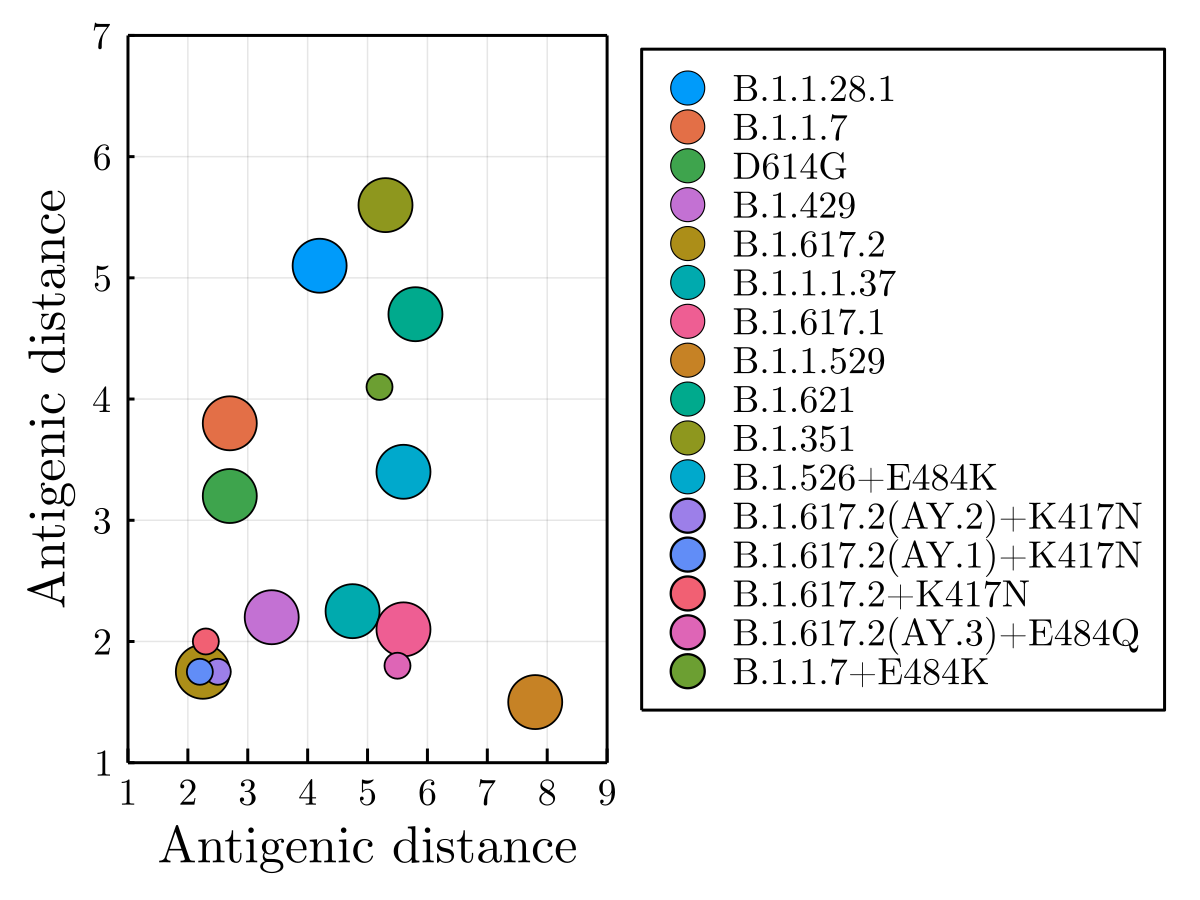
\includegraphics[width=0.5\textwidth]{../SarsEvoModel/plots/antigenic_map_paper.png}
    \caption{Antigenic cartography of Sars-CoV-2, reproduced from \cite{wilksMappingSARSCoV2Antigenic2022}, Fig. 2}
\end{figure}
\end{column}

\end{columns}
\end{frame}
\begin{frame}{Model parameters/variables}
    \begin{table}[h!]
        \begin{center}
        \begin{tabular}{c|p{8cm}}
                Symbol & Description \\
                \hline
                \hline
                $N$ & Size of variant grid \\
                $S_{ij}$ & Population susceptible to variant $(i,j) \in [0,N]^2$ \\
                $I_{ij}$ & Population infected by variant $(i,j) \in [0,N]^2$\\
                $R_{ij}$ & Recovered/Immune to variant $(i,j) \in [0,N]^2$\\
                $\sigma_{ijkl}$ & Probability that exposure to variant $(i,j)$ causes immunity \newline to variant $(k,l)$\\
                $\beta_{ij}$ & Transmission rate of variant $(i,j)$\\
                $\xi$ & Recovery rate of all strains \\
                $\gamma$ & Rate of immunity loss of all strains \\
        \end{tabular}
        \caption{Table of symbols for Model 2}
    
        \label{variables_2}
        \end{center}
    \end{table}
    In practice, we assume $\sigma_{ijkl}$ is just a 2-D gaussian distribution parameterized by the distance between $(i,j)$ and $(k,l)$.
\end{frame}
\begin{frame}{Model Equations}
    \small
    \begin{equation}
        \frac{S_{ij}}{dt} = -\sum_{kl} \beta_{kl} \sigma_{ijkl} S_{ij} I_{kl} + \gamma R_{ij}  \label{Seqn}
    \end{equation}
    \begin{equation}
        \frac{ I_{ij}(t)}{dt} = \beta_{ij} S_{ij} I_{ij} - \xi I_{ij} + M \left(- 4I_{ij} + I_{i-1,j}  + I_{i+1,j} + I_{i,j-1} + I_{i,j+1} \right) \label{Ieqn}    
    \end{equation}
    \begin{equation}
        \frac{R_{ij}(t)}{dt} = \xi I_{ij} - \gamma R_{ij}  \label{Reqn}
    \end{equation}

    Boundary conditions: $I_{0,j} = 0, I_{j,0} = 0,  I_{N,j} = 0, I_{j,N} = 0$

    Initial conditions computed from genomic data in GISAID 
\end{frame}
\begin{frame}[allowframebreaks]

\bibliographystyle{apalike}
\bibliography{ref.bib}
\end{frame}

\end{document}